\documentclass[a4paper,12pt]{article}
\usepackage{mathtools, amsmath, listings,graphicx}
\graphicspath{ {images/} }
\begin{document}
\lstset{language=Python}

\title{Paths: a Powerful Graph Invariant with Interesting Limitations}
\author{Grady Ward}

\maketitle

In searching for a polynomial time-complexity solution to the graph isomorphism problem, many researchers have focused on, \emph{vertex invariants}, numerical properties calculated over a vertex of a graph that can be deterministically calculated, regardless of how the graph is represented or labeled. This article will aim to describe the descriptive power and information density of the \(Paths(p, v)\) function, a vertex invariant that counts the number of closed paths of length \(p\) through a vertex \(v\). The \(Paths\) function, in order to be applied to the graph isomorphism problem, is used to construct an algebraic graph invariant, with the application of sorting to the results of individual vertex \(Paths\) results.

Though research into the descriptive power of this function has shown that it does not fully determine the graph, the lines of inquiry have proven to be fruitful in describing patterns of graph behavior that a casual observer would not anticipate.  Additionally, the invariant's descriptive power can be computationally described in a way that is meaningful, and shows that for its time complexity, it is an incredibly discriminatory algorithm.  Finally, this article will hope to address the various lines of inquiry that will hopefully be addressed in further research on this topic, including a systematic analysis of the classes of graphs that the Paths function is effective for, and those for which it is insufficient to prove isomorphism.

\section{Background}

To begin a discussion of this work, we must first establish a mutual understanding of the functions that we are discussing, the scope of existing research on this topic, and an appropriate category of graphs to examine.

\subsection{Definitions}

In this analysis, we will be examining \(undirected\) graphs that do not contain multi-edges nor loops.  Any graph under these three constraints can be represented as a symmetric adjacency matrix, with zeros along the diagonal, and ones or zeroes in the remaining locations denoting an edge or disjoint vertices respectively. We will regularly reference this matrix as \(A\) with no additional annotation.

The vertex invariant we are going to examine (\(Paths(p, v)\)) is the number of closed paths of a length \(p\) that contain the vertex \(v\). A path is a sequence of vertices such that each vertex shares an edge with the next one. A Path can be notated by the sequence of the vertices that are visited (e.g. ABCDE or BACAB). A Path is \emph{closed} if the first and last vertex in their traversal sequence are the same. Note that though \(ABCDE\) and \(EDCBA\) describe the same edges, they are distinct paths: even though an undirected graph doesn't have directional edges, paths maintain the order of the edges they traverse.

For this article, when we describe a path as a geometric polygon (such as a triangle, quadrilateral, pentagon, etc.), we will define to be a closed path such that the vertices of the path are non-repeating (aside from the first and last, as we assume that it is closed). Thus, \(ABABA\) does not form a quadrilateral, even though it is a closed path of length four. Note that this path could equally well be described as \(BABAB\), as closed paths are inherently cyclic, and do not demand a starting vertex.  Additionally, we will assume that unlike a path, a polygon's directionality does not matter (thus the polygon ABCA is the same as the polygon ACBA). 

\subsection{Computation of the Paths Function}

The \(Paths(p, v)\) function counts the number of unique closed paths that pass through a given vertex, \(v\).  This information can be easily computed using \(A\). Just as the entries of \(A^1\) represent the existence of paths of length 1 between two vertices (edges), the entries of \(A^p\) represent the number of paths of length \(p\) between any two vertices (by examining the row and column corresponding to two vertices). Thus, to find the number of closed paths of length \(p\) that contain a given vertex \(v\), we simply need to calculate: \[Paths(p, v) = A^p[v, v]\]Where \(v\) is being used interchangeably here with its represented position within the adjacency matrix. Thus, calculating a specific value of \(Paths(p, v)\) can occur in the time it takes to exponentiate \(A\) to the power \(p\).  Though it is a well known result that matrix multiplication can be done in faster than \(O(n^3)\) time, we will be using the na�ve assumption that matrix multiplication runs in \(O(n^3)\) in order to make the computational complexity calculations more accessible.  Under that assumption, it is clear that calculating \(Paths(p, v)\) will occur in \(O(pv^3)\) time. This is well within polynomial time, so long as we request a polynomial number of values from \(Paths(p, v)\). Thus we can consider this invariant one in the traditional vein of looking for polynomial invariants with the broad aim of solving GI in polynomial time, though we have already established that it does not uniquely determine isomorphism.

\subsection{Expansion to a Paths Object}

Since \(Paths(p, v)\) is a function that operates over a vertex, we will be examining a slightly modified version of the function which operates over a graph: \(Paths(P, G)\).  \(Paths(P, G)\) produces a graph invariant that is related to its vertex invariant function by a simple translation.  \(Paths(p, v)\) is calculated for all \(v\in G, p \leq P\), resulting in \(v\) vectors, each of which has \(P\) elements, representing the paths function when calculated at that node for each successive value of \(p\). Since vectors are comparable objects, we can sort them, and return back a list of these vectors as a graph invariant, one that is computable and invariant to changes in vertex relabeling or adjacency matrix ordering. A skeptical reader should convince themselves that this holds true, even when two of the vectors to be sorted are identical, the resulting \(Paths\) object is valid and deterministically constructed from the graph.

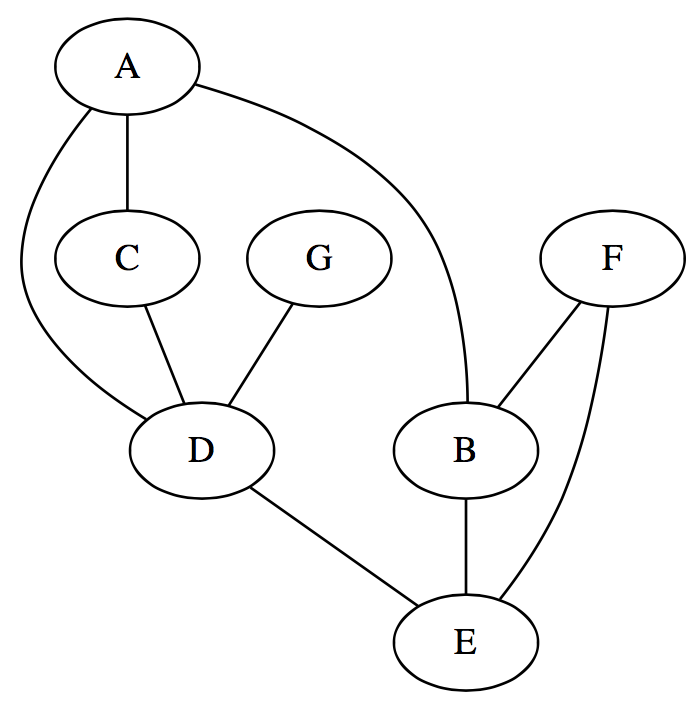
\includegraphics[scale=0.4]{examplegraph}
\( A = \left ( \begin{array}{ccccccc}
0 & 1 & 1 & 1 & 0 & 0 & 0 \\1 & 0 & 0 & 0 & 1 & 1 & 0 \\1 & 0 & 0 & 1 & 0 & 0 & 0 \\1 & 0 & 1 & 0 & 1 & 0 & 1 \\0 & 1 & 0 & 1 & 0 & 1 & 0 \\0 & 1 & 0 & 0 & 1 & 0 & 0 \\0 & 0 & 0 & 1 & 0 & 0 & 0\end{array} \right)\) 

\subsection{Co-Paths and Isomorphism}

Finally, two Graphs are said to be Co-Paths if they produce the same \(Paths\) object.  Since the Paths function is invariant to labeling and positioning, all isomorphic graphs are Co-Paths. However, a broader question is implied by this implication: does the reverse hold? Does Co-Paths determine isomorphism?  The answer turns out to be no, but the line of inquiry that leads to this result is worth examining, and leads us to a broader understanding and appreciation for the discriminatory power of the \(Paths\) function with respect to isomorphic graphs.


\section{Cardinality Analysis}

An obvious choice in attempting to verify a bijection is the analysis of the cardinality of the target and domain spaces.  If a function maps all inputs to a space of equal size as its own, it must be a bijection.  Thus, in pursuing to quantify the relationship between the \(Paths\) object and the isomorphism relationship, I set about examining the cardinality of two sets: the set of all non-isomorphic graphs, and the set of all achievable \(Paths\) objects.

Note that this line of inquiry is what allowed us to rule out that the two relationships are the same. If we were able to prove that the relationship between the \(Paths\) objects and the set of all graphs was linked by a bijective function, we would have proven that if two graphs agree on their corresponding Paths's matrix, then they are the same graph. This would have been valuable because \(Paths\) objects can be directly compared and sorted, while graphs cannot immediately be compared in polynomial time by any currently understood algorithm.

How to we go about calculating the cardinality of both sets?  Luckily, the cardinality of the first set is well established.  The series A000088 in the online encyclopedia of integer sequences gives us the number of non-isomorphic graphs up to N=28.  Now to calculate the number of distinguishable paths matrices of a given order, I turned to programming, with various degrees of success. Below are the various results of these computations, and a brief overview of their implementation and success rates.

\subsection{Brute Force - Java}

Start with what you know.  As early as October, I had written a simple function in Java that computed the number of unique paths vectors by doing raw calculation of paths Matrices, sorting using a simple row comparison, and a tree set to do comparison of paths objects.  Attempting to approach this problem from the most naive standpoint first, I didn't make any smart or deductive assumptions about the number of graphs that are non-isomorphic, but instead chose to process every single adjacency matrix of a given size.  Though the number of graphs of a given size is exponentially defined, the number of potential representations of those graphs has an even steeper exponential growth rate. 

The final result of this line of inquiry appeared to corroborate the strength of the paths function, at an exorbitant computational cost.  Running on a Macbook Air with a 1.7 gHz processor and 8 GB of RAM, this calculation took 28 hours to complete, and only described the cases with eight or fewer vertices. Far from ideal.  For \(V <= 8\), this analysis calculated that the number of valid paths objects of the same size exactly matched the A000088 sequence.  Going forward with more advanced computations, we knew already that we would not find non-isomorphic co-paths graphs with fewer than nine vertices.

\subsection{NAUTY Package}

Thankfully, the generation of non-isomorphic graphs is well studied, and practical algorithms have been developed for their systematic enumeration.  One of the best is the \emph{geng} graph generator that is offered as part of the \emph{NAUTY} package, written in C.  Though computation of these graphs is still exponentially asymptotic, it is orders of magnitude faster than brute force calculations.  The NAUTY package saves its graphs in a format called Graph6, which allowed us to efficiently store all possible graphs of a given cardinality and vertex count in a line delimited file, to split up the tasks of generating and processing the graphs.

All computations beyond this point were done in this way: a set of files were generated of the form [NVERTICES]-[NEDGES].txt, which stored the Graph6 format of the adjacency matrix for all non-isomorphic graphs matching those computational descriptions.

\subsection{GPU Calculations}

Of growing importance in scientific computing is the role of GPUs in large and distributed computation.  With a twofold agenda (education and performance), I set out to utilize GPU arrays in the computation of \(Paths\) by using established protocols for matrix multiplication in OpenCL.  The result was successful in outperforming a traditional implementation in C by a factor of four, but unfortunately was not fully parallelizable.  I am hoping to work next semester to consider broader applications of the GPU to actual \(Paths\) computation, collection, and comparison, in a way that takes advantage of the massive parralellizability of this problem, while trying to find creative ways to get around the highly limiting nature of the memory access procedures that differentiate GPU programming from CPU multithreading. 

\subsection{C Calculations}

Now, most of my work on this project has been theoretical, but this piece in particular has been of great algorithmic and pragmatic interest and education.  After somewhat abandoning the GPU as the method by which to speed up these calculations, I decided to try to use custom C to maximize my memory efficiency and attempt to do the minimal amount of computation necessary to be successful. What resulted is probably the best piece of code that I have ever written, and it reflects many facets of my education in computer science here at Brandeis: stream processing, advanced data structures, intentional bit manipulation, and memory allocation and reuse.

The program maintains a Trie, where the input to the Trie is the Paths object's sorted vector elements in increasing levels of power. This is far from revolutionary.  What was incredibly powerful about this technique was the way in which I used stream processing to delay computation and comparison of Graphs.

When inserted into the Trie, a new graph element would only compute the first level of its exponentiated form (i.e. \(A^2\)).  It would store this value (a running matrix with its current exponentiated power of \(A\)) alongside the graph within a structure which also included an elaborate (but low memory) mechanism to allow individual number output of the next number to be used in insertion into the trie (or the next level of the trie). This second part is particularly non-trivial because we have to consider past sorting decisions in making present sorting decisions, and have to store the results of those decisions in a fashion that is memory efficient and computationally easy to manipulate. My code here is particularly thoughtful, and uses a quadratic runtime (in the number of vertices) in exchange for a cubic amount of space.

Finally, when a new graph is inserted into an existing trie node, if there already exists a graph within that node, the original inhabitant is kicked out, and both are re-inserted into that node.  This means that we only exponentiate the matrix (an \(O(n^3)\) operation) the minimal number of times necessary to differentiate between graphs.  On average, this means that rather than exponentiating a matrix \(V\) times in the naive version, we average \(0.2V\) matrix exponentiations, a five fold speed increase in multiplication alone. The number of comparisons in this methodology can also prove to be minimal, and using a trie structure over a comparable tree led to an enormous speed up in efficiency, wile still having a depth that is guaranteed to be a linear factor of the result (which is generally a linear function of the input, but not for all cases). 

The result of this work, in addition to the pre-computation of non-isomorphic graphs through the NAUTY package was a program which could perform the same task as the Java function in under 2 seconds, and could expand upon the performance to \(V=10\) with all computations under 20 seconds.  This aspect of the project is a great point of personal pride and growth, and demonstrates the value of a careful consideration of algorithms and data structures in scientific computation. 

\section{Theoretical Analysis}



\section{Future Lines of Inquiry}

When attempting to prove that a function is a bijection, cardinality analysis can prove empirically that it is, regardless of the internal mechanisms of the functions or its operating domain and range. We will use this type of analysis to construct proof for a bijection of our paths function on small graphs. The Paths function can be thought of as a function which operates between two sets: the set of all graphs, and the set of all possible Paths matrices.  

Since I have not yet defined paths matrices I will here.  Previously discussed was how the paths function is operated on an individual vertex within a graph, and returns a vertex invariant which is a 1xP vector which reflects the state of that vertex and its surroundings.  Compiling these vectors for each one of our vertices assembles us V vectors of size P.  Since vectors are inherently comparable, we can sort them.  Then appending them together creates a matrix of size VxP, where the paths function for each vertex is placed in a given position regardless of its original positioning within the adjacency matrix.

Thus, we are defining our second set to be the set of all such possible paths matrices.  It should be clear that the function Paths, mapping from a graph to such a mathematical object, is injective, as the cardinality of the domain could not be smaller than the cardinality of the range.  However, the question remains: is it a bijection? Why is this important?

If we were able to prove that the relationship between the Paths matrices and the set of all graphs was linked by a bijective function, we could prove that if two graphs agree on their corresponding Paths's matrix, then they are the same graph. This is valuable because paths matrices can be directly compared and sorted, while graphs cannot immediately be compared in polynomial time (which is what this article is attempting to redress).

So how to we go about calculating the cardinality of both sets?  Luckily, the cardinality of the first set is well established.  The series A000088 in the online encyclopedia of integer sequences gives us the number of non-isomorphic graphs up to N=28.  Now to calculate the number of distinguishable paths matrices of a given order.

\end{document}